\section{Tuning methods}
Different methods can be used to tune a PID controller as the, Zieggler-Nichols, Skogestad and Good Gain method, having in common the same goal : get a fast response and provide a desired stability.\par
As a first try, a PID controller was designed using the Good Gain method. Later, a comparison between P, PI, PD and PID controllers was performed with the \emph{PID Simulink} box, in order to choose the most effective one for our application.\par 	

\subsubsection{The Good Gain}


The structure of the controller can be seen on the figure below. Taking as input the error angle \textbf{$\theta_{e}$} and outputting the required voltage \textit{V}, which is after limited by a saturation box to supply the motor, this controller has the final task of converting a value in radian into voltage.\par

\begin{figure}[H]
  \centering
  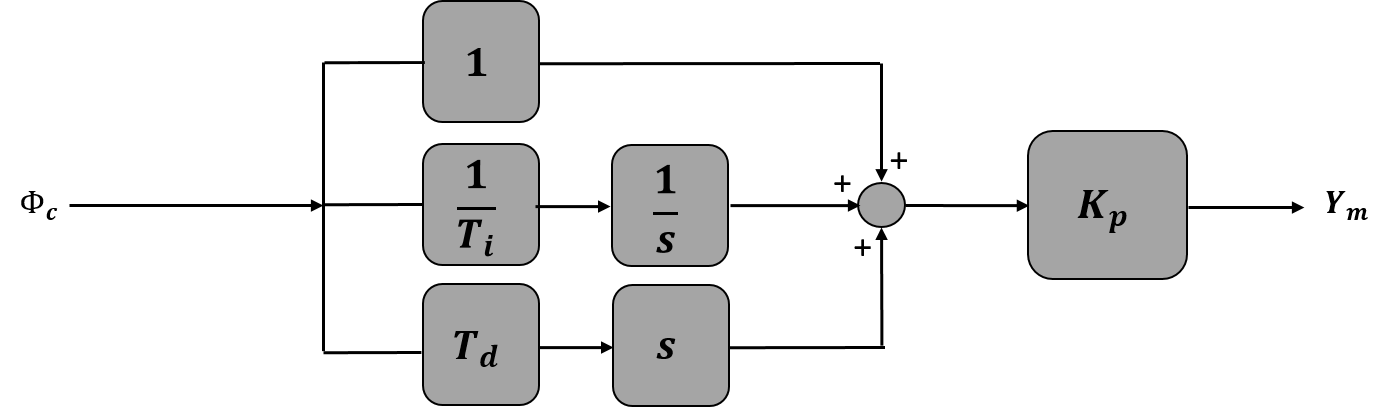
\includegraphics[scale=0.5]{figures/controller_model.png}
  \caption[LABEL] {Block diagram of the PID controller}
\end{figure}
  
This method can be split up in three different parts. In the first part it is supposed to set the proportional parameter. Thus, choosing $T_i$ = $\infty$ and $T_d$ = 0 (respectively the integral and the derivative term to zero), results in the step from the figure \ref{fig:subim11}.
\begin{figure}[H]
\hfill
\subfigure[Set Ti = inf , Td = 0 and Kp = 1]{
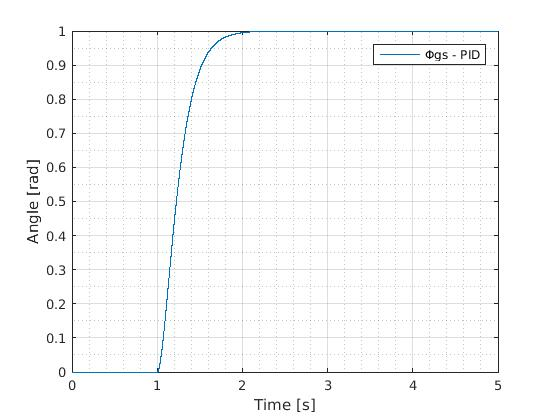
\includegraphics[scale=0.3]{figures/GG1.jpg}
\label{fig:subim11}}
\hfill
\subfigure[Increase Kp until finding a slight overshoot but a well damped response]{
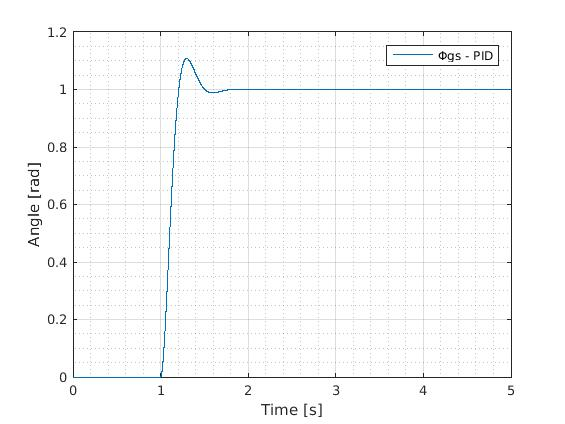
\includegraphics[scale=0.3]{figures/GG2.jpg}
\label{fig:subim12}}

\caption{Good Gain : Setting the propotional parameter}
\end{figure}


Increasing $K_p$ in figure \ref{fig:subim12} will allow to reduce the rising time. Morover, changing this proportional gain is a needed step to find a slight overshoot and a well damped response. Hence, having an overshoot and the first undershoot, $T_{out}$ can be defined, being the time between the peak of the overshoot and the one of the undershoot.\par
\vspace{5mm}
Adding the integral parameter implies a relation with the previous defined time between the peak of the overshoot and undershoot. Thus, $T_i = 1.5T_{out}$. The objective of this step \ref{fig:subim13} is to eliminate the steady state error.



\begin{figure}[H]
\hfill
\subfigure[Set Ti = 1.5$\cdot T_{out}$]{
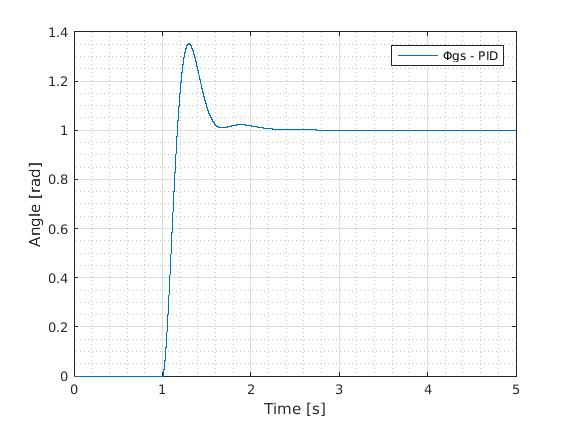
\includegraphics[scale=0.29]{figures/GG3.jpg}
\label{fig:subim13}}
\hfill
\subfigure[Set Td = $\frac{Ti}{4}$]{
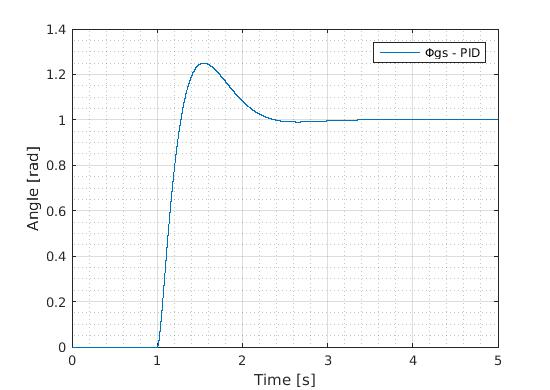
\includegraphics[scale=0.31]{figures/GG4.jpg}
\label{fig:subim14}}
\hfill

\caption{Good Gain : Adding integral and derivative parts}
\end{figure}

At this point, the controller is a proportional-integral. The high overshoot resulting from adding the integral term can be attenuated by setting the derivative part, shown in figure \ref{fig:subim14}. The gain $T_d$ will act as a damper on the system and therefore reduce the high variations of the step response. In the Good Gain method, this value is described to be $T_d = \frac{T_i}{4}$.

\vspace{5mm}

Theoretically, the tuning of the controller using the Good Gain method is done. However, it is possible to improve the controller based on the application that is wanted. In the case of this project, stability and minor overshoot was more important than the reaching speed of the reference value. Therefore, based on the principles seen in sections \ref{sec:pid_theory}, the overshoot of the system was attenuated, the undershoot cancelled and the drop-off smoothed (figure \ref{finalGG}).

\begin{figure}[H]
  \centering
  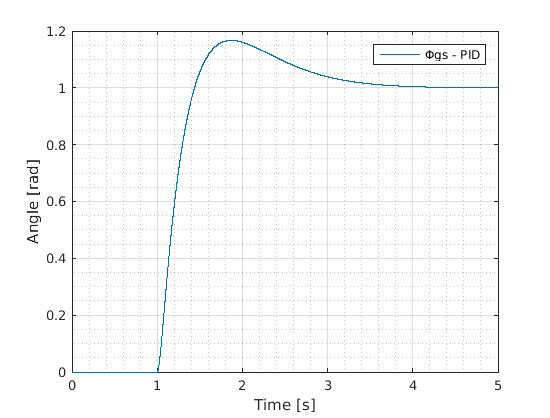
\includegraphics[scale=0.5]{figures/GG5.jpg}
  \caption[LABEL] {Good Gain : final settings}
  \label{finalGG}
\end{figure}

However, the time needed to tune and the uncertainties of the different steps and results were the weaknesses of this method. For instance, as described in figure \ref{fig:subim12} , a "slight overshoot" is a parameter that can be relative depending on the designer.\par  
  
\subsubsection{PID Simulink box}
The PID simulink box is an interesting alternative to the good gain method to tune a controller. As a matter of fact, the previous described method has its own limits.\par 
  
Therefore, the PID simulink box, that includes an automatic tuning tool and a real time response of the system, was a suitable option to tune the controller. Futhermore, this technique incorporates a fourth parameter in its PID model, as shown in figure \ref{PID_box_N}. 
 
\begin{figure}[H]
\centering
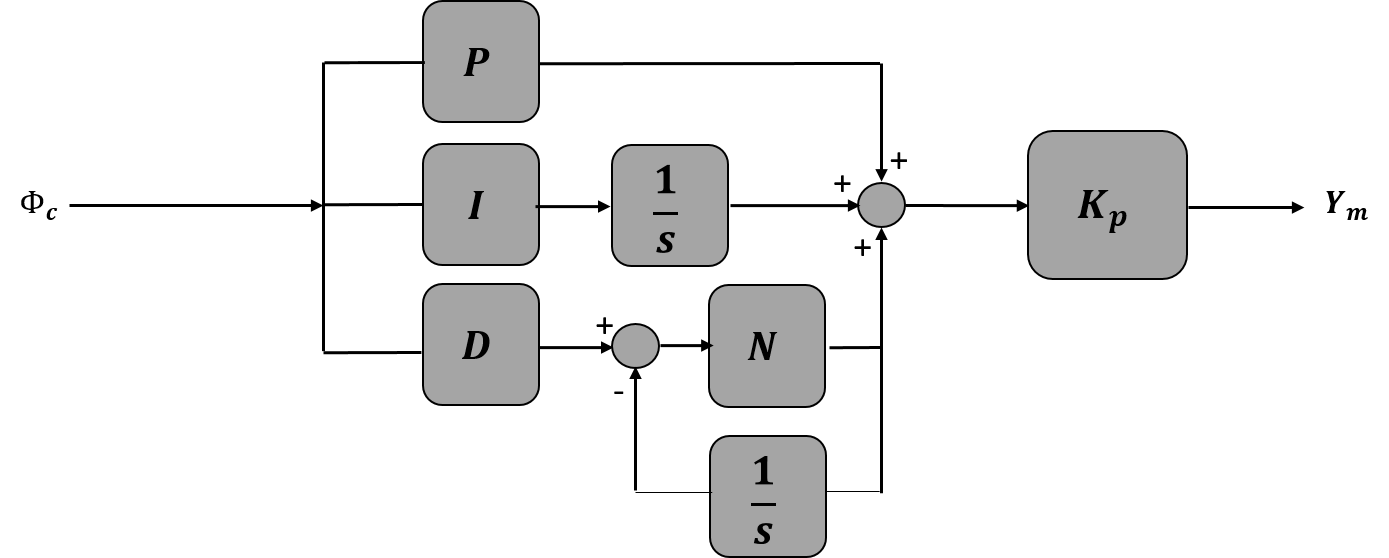
\includegraphics[scale=0.4]{figures/controller_box.png}
\caption{Inside of the PID box}
\label{PID_box_N}
\end{figure}

The added parameter is the filter coefficient, \textit{N}, applied on the derivative term of the controller. Thus, its transfer function becomes \ref{eq:N_PID}

\begin{equation}\label{eq:N_PID}
H(s) = P + I\frac{1}{s} + D\frac{N}{1+N\frac{1}{s}}
\end{equation}

Including the N term avoids a 'pure derivative' that reacts easily to noises. Thus, the filter coefficient, being the pole location of the filter in the derivative action, transforms this part of the controller into a low pass filter. Hence, the bandwidth of the filter can be chosen by changing the N value.\par

\vspace{5mm}


The PID tuner considers as the plant all blocks in the loop, that can include linearities and nonlinearities, between the controller output and input. Then, the PID tuner automatically linearizes the plant at the operating point based on the initial conditions of the model. This process works as an approximation to the nonlinear system and is valid in a small region around its operating point.\par

The gains of the PID controller are calculated based on three different concepts: closed-loop stability, adequate performance and adequate robustness. The closed-loop stability means that the system’s output remains bounded for a bounded input. The adequate performance of the PID controller will allow the system to track reference changes and suppress disturbances as rapidly as possible. Finally, the robustness is the property that takes into account the gain and phase margin in order to allow for modelling errors or variations in system dynamics. Thus, as is referred in the MathWorks webpage, the algorithm for tuning PID controllers meets these objectives by tuning the PID gains to achieve a good balance between performance and robustness.



